\section{Equazioni alle differenze}
I LTI causali a tempo discreto possono essere rappresantati in modi differenti, tra cui la combinazione lineare con coefficienti costanti nel tempo (invariante). 

Il comportamento di un sistema LTI a tempo discreto e causale può essere descritto anche da equazioni alle differenze, come visto precedentemente:
$$y(n) = -\alpha_1y(n-1) - \alpha_2y(n - 2) - \dots - \alpha_My(n - M) + \beta_0x(n) + \beta_1x(n - 1) + \dots + \beta_Nx(n - N)$$
$$y(n) = \sum_{k=0}^{N} b_kx(n - k) - \sum_{j=1}^{M} a_jy(n - j)$$
Si ricorda che i coefficienti sono costanti e indipendenti dal tempo, per assicurare la stazionarietà. Un'equazione è detta ricorsiva se almeno un coefficiente $a_i$ è diverso da zero.

Quando il sistema ha una parte ricorsiva, dipende di fatto da più istanti precedenti dell'input, e non solo dai $N$ istanti evidenti dalla sommatoria. $M$ è l'ordine dell'equazione alle differenze (ordine del sistema).

Il ritardo su $y$ indica di che ordine è il sistema: il primo ordine, per esempio, ha ricorsione con un campione in ritardo. 

L'output di un sistema ricorsivo dev'essere calcolato in sequenza, al contrario di un sistema non ricorsivo in cui i campioni possono essere valutati con qualsiasi disposizione.

Esempi di sistemi:
\begin{itemize}
	\item Identità $y(n) = x(n)$, non ricorsivo e causale;
	\item Ritardo (anticipo) unitario $y(n) = x(n \pm 1)$, non ricorsivo e (non) causale;
	\item Media mobile $y(n) = \frac{1}{3} [x(n - 1) + x(n) + x(n + 1)]$, non ricorsiva e non causale;
	\item Accumulatore $y(n) = \sum_{-\infty}^{n} x(k)$, causale ricorsivo con memoria infinita.
\end{itemize}
In quest'ultimo caso, l'output a un istante $n$ dipende dal valore dell'input per tutti gli istanti precedenti, cioè dall'output ricavato con essi: bisogna conoscere anche le condizioni iniziali $y(n - 1)$.

Se il sistema accumulatore $y(n) = y(n - 1) + x(n)$ non ha subito alcuna eccitazione prima dell'istante $n$, $y(n - 1) = 0$ e il sistema è scarico (per $n = -\infty$).

\subsection{Diagrammi a blocchi}
Ogni operazione di cui è composto un sistema viene rappresentata in un diagramma a blocco, che contiene eventualmente anche una parte ricorsiva (freccia all'indietro). Si ricordano la linearità e la commutatività.
\begin{figure}[h]
	\centering
	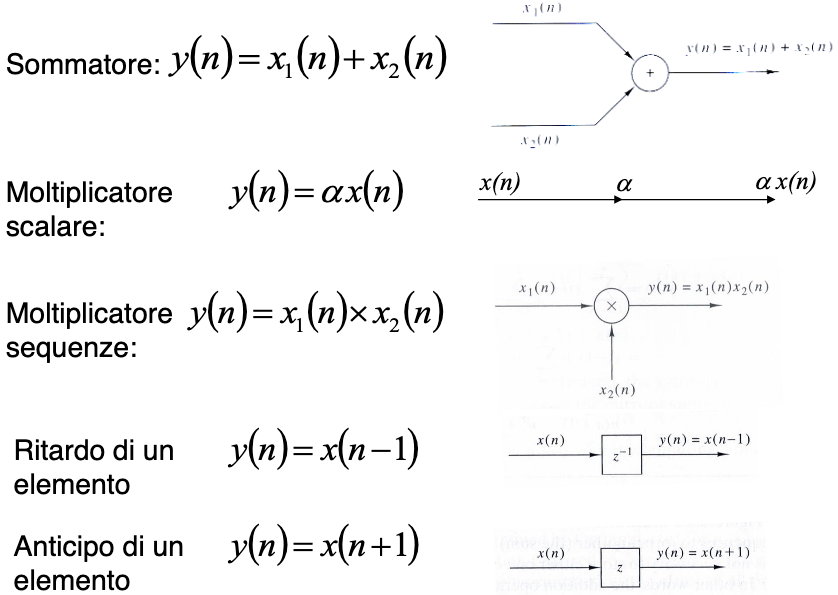
\includegraphics[scale=0.4]{Lezioni/Immagini/blocchi}
\end{figure}

\subsubsection{Media cumulativa}
La media cumulativa è un sistema ricorsivo non stazionario, con normalizzazione effettuata in base a un parametro non costante. 
$$y(n) = \frac{1}{n+1} \sum_{k=0}^{n}x(k)$$
Il calcolo di $y(n)$ richiede la conoscenza di tutti i valori di $x(n)$ precedenti, ma può essere semplicemente calcolato da $y(n-1)$, cioè il precedente output e l'input corrente: il valore di $y(n_0)$ si calcola a partire da una sequenz di input applicata per $n \geq n_0$ e dalla condizione iniziale $y(n_0 - 1)$.
$$(n + 1) y(n) = \sum_{k=0}^{n} x(k) + x(n) = ny(n-1) + x(n)$$
$$y(n) = \frac{n}{n+1} y(n-1) + \frac{1}{n+1} x(n)$$

\begin{figure}[h]
	\centering
	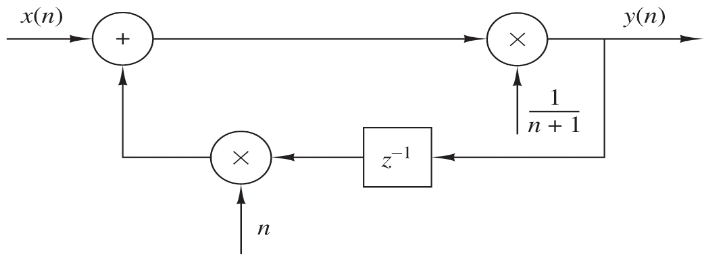
\includegraphics[scale=0.4]{Lezioni/Immagini/media}
\end{figure}

\newpage
\subsubsection{Radice quadrata}
Questo sistema calcola la radice quadrata in modo ricorsivo, a partire da una condizione iniziale $y(-1)$ che approssima il valore cercato. Al crescere di $n$, la stima del valore migliora.
$$y(n) = 0.5 \frac{x(n)}{y(n-1)} + 0.5y(n-1)$$
La radice quadrata non è un sistema lineare: non esistono sommatorie, ma il termine $y$ compare al denominatore quindi non è rappresentabile come combinazione lineare. 

\begin{figure}[h]
	\centering
	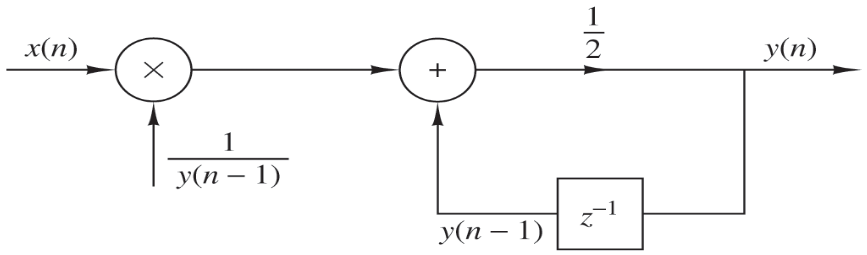
\includegraphics[scale=0.3]{Lezioni/Immagini/radice}
\end{figure}

\section{Risposta all'impulso}
La risposta all'impulso viene descritta attraverso un prodotto di convoluzione, come sequenza finita o infinita. I primi casi non hanno la ricorsione, sono campioni combinati con pesi: i valori di $h$ sono i coefficienti di $x$.

In base alla risposta all'impulso, i sistemi possono essere divisi in due gruppi: FIR (Finite Impulse Response) e IIR (Infinite Impulse Response). 

\subsection{FIR}
$$h(n) = \begin{cases}
\neq 0 & \quad 0 \leq n \leq M - 1 \\
= 0 & \quad n < 0 \land n \geq M
\end{cases}$$

La risposta di un sistema FIR a un generico segnale è allora:
$$y(n) = x(n) * h(n) = \sum_{i = 0}^{\infty} h(i)x(n - i) = \sum_{i = 0}^{M-1} h(i) x(n - i)$$
Per un sistema FIR, l'output a qualsiasi istante $n$ è semplicemente la somma di una combinazione lineare pesata degli $M$ valori più recenti della sequenza di input.

Il sistema agisce come una finestra che vede solo $M$ valori recenti, quindi ha memoria $M$. \\
I sistemi FIR possono essere sempre realizzati in modo non ricorsivo, essendo in funzione di $M$ campioni pesati per la risposta all'impulso $h(n)$. Questo deriva dal fatto che una LTI non ricorsiva dipende solo da un numero finito di istanti nel passato.

\subsection{IIR}
$$h(n) = \begin{cases}
\neq 0 & \quad n \geq n_0 \\
= 0 & \quad n < n_0
\end{cases}$$

La risposta di un sistema IIR causale a un generico segnale è allora:
$$y(n) = x(n) * h(n) = \sum_{i = 0}^{\infty} h(i)x(n - i)$$
L'output a qualsiasi istante $n$ dipende da tutti i valori della sequenza di input: il sistema ha memoria infinita e non è realizzabile, perché richiederebbe infinite locazioni di memoria. 

Se la sommatoria va a infinito, non c'è una diretta corrispondenza con il dominio delle frequenze, quindi non si individua $y(n)$ guardando la risposta ma si utilizzano le equazioni alle differenze e il dominio trasformato.

\subsubsection{Prima forma diretta}
Realizza un'equazione lineare alle differenze del primo ordine a coefficienti costanti, utilizzando due unità di ritardo (memoria) distinte come se fossero due sistemi a cascata. Il primo sistema non è ricorsivo, mentre il secondo lo è.
$$y(n) = -\alpha_1y(n-1) + \beta_0x(n) + \beta_1x(n-1)$$
Per la proprietà commutativa, scambiando l'ordine dei sistemi il risultato non cambia, ma è necessario introdurre una variabile ausiliaria.
\begin{figure}[h]
	\centering
	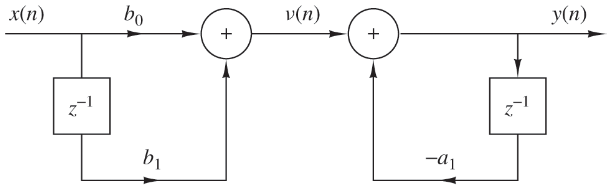
\includegraphics[scale=0.4]{Lezioni/Immagini/diretta1}
\end{figure}

\subsubsection{Seconda forma diretta}
$$\omega(n) = -\alpha_1\omega(n-1) + x(n) \qquad y(n) = \beta_0\omega(n) + \beta_1\omega(n-1)$$
Le due unità di ritardo hanno entrambe in input $\omega(n)$ e in output $\omega(n-1)$, e possono quindi essere rappresentati con un'unica unità di ritardo. Ciò è efficiente nelle applicazioni pratiche in termini di memoria. 
Il passaggio dalla prima forma diretta alla seconda si può estendere al caso di una generica equazione alle differenze di ordine $N$:
$$y(n) = \sum_{k=0}^{M}\beta_kx(n-k) - \sum_{j=1}^{N}\alpha_jy(n-j)$$

\newpage
Ciò richiede $N + M$ unità di ritardo e $M + N + 1$ moltiplicazioni. La seconda forma diretta è data dalla cascata di un sistema ricorsivo seguita da uno non ricorsivo, con $max(N, M)$ ritardi.
\begin{figure}[h]
	\centering
	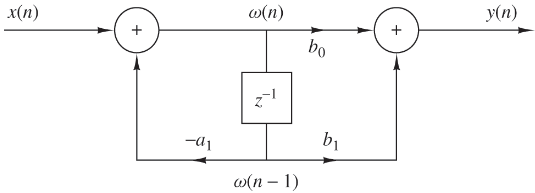
\includegraphics[scale=0.4]{Lezioni/Immagini/diretta2}
\end{figure}
